\documentclass[12pt, a4paper]{article}

\usepackage{graphicx}
\usepackage{amsmath}

\begin{document}

\tableofcontents
\newpage

\section{Problem 1 : Introduction}
\subsection{Description}

F5 : $ab^x$ is an exponential function, where a is a constant value, $a \ne 0$ and it also represents starting (initial) value , b is called base and is a positive real number and $b \ne 1$, x is called the exponent (power), it is independent variable . In this function, b is a constant value, whereas x is variable.

\subsection{Domain}

The domain for exponential function is the set of real numbers. 
\newline $x \in R$ ,  -$\infty < x <\infty$ , Domain : $\{x \mid x \in R$\}

\subsection{Co-Domain}

Co-Domain is the set of all possible function output values.
\newline Suppose $y = f(x) = ab^x $, then -$\infty < y <\infty$ , so the range will be $[-\infty,\infty]$.

\subsection{Characteristics}
\begin{itemize}
    \item In exponential function, if $ b > 0 $, then it is known as exponential growth function (increasing function). Its graphical representation shown in the left part of the figure 1.
    \item In exponential function, if $ 0 < b < 1$, then it is known as exponential decay function (decreasing function). Its graphical representation shown in the right part of the figure 1.
    \item Exponential function have horizontal asymptote (i.e function approaches to a imaginary horizontal line but never crosses) at $ Y=0 $ (i.e $ X $ – axis).
    \item They are continuous function.
    \item There is no symmetry in exponential function, so they are neither odd nor even function.
    \item Exponential function is not injective but is surjective. 
\end{itemize}

\newpage

\begin{figure}[h]
  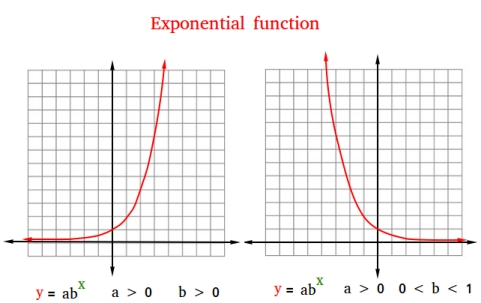
\includegraphics[width=\linewidth]{exponential-function.jpg}
  \caption{Exponential Function Graph (Growth And Decay).}
  \label{fig:exponential function graph (growth and decay)}
\end{figure}

\subsection{Context of Use Model}
\begin{figure}[h!]
  
\includegraphics[width=0.5\linewidth]{frog.jpg}
  \caption{Exponential Function Graph (Growth And Decay).}
  \label{fig:exponential function graph (growth and decay)}
\end{figure}


\newpage

\section{Problem 2 : Requirements}
\begin{enumerate}
    \item{} Requirement 1
        \begin{itemize}
        \item \textbf{ID} : R1
        \item \textbf{Version} : 1.0
        \item \textbf{Type} : Functional Requirement
        \item \textbf{Priority} : High
        \item \textbf{Difficulty} : Easy
        \item \textbf{Description} : In the exponential function $ ab^x $, the input value a should be greater than 0 i.e., $ a > 0 $ (or else it will result in output of the function to be 0 for every input), also input value of base b must be greater than 1 i.e., $ b > 1 $ (or else if $b = 1 $, it will result in output of the function to be ‘a’ for every input of x).
        \end{itemize}
    
    \item{} Requirement 2
        \begin{itemize}
        \item \textbf{ID} : R2
        \item \textbf{Version} : 1.0
        \item \textbf{Type} : Functional Requirement
        \item \textbf{Priority} : High
        \item \textbf{Difficulty} : Easy
        \item \textbf{Description} : In the exponential function $ab^x$, the input value of base b must not be negative as it will result will be complex numbers so $b > 0$.
        \end{itemize}
    
    \item{} Requirement 3
        \begin{itemize}
        \item \textbf{ID} : R3
        \item \textbf{Version} : 1.0
        \item \textbf{Type} : Functional Requirement
        \item \textbf{Priority} : High
        \item \textbf{Difficulty} : Easy
        \item \textbf{Description} : : In the exponential function $ab^x$, the input value of x must be any real number. i.e $x \in R$.
        \end{itemize}
    
    \newpage
    
    \item{} Requirement 4
        \begin{itemize}
        \item \textbf{ID} : R4
        \item \textbf{Version} : 1.0
        \item \textbf{Type} : Functional Requirement
        \item \textbf{Priority} : High
        \item \textbf{Difficulty} : Medium
        \item \textbf{Description} : The system must take input values of a, b and x from the users and return the output of $ab^x$ function. For example, if $ a = 2, b = 3 , x = 2,$ the output should be $ 18 $.
        \end{itemize}
    
    \item{} Requirement 5
        \begin{itemize}
        \item \textbf{ID} : R5
        \item \textbf{Version} : 1.0
        \item \textbf{Type} : Functional Requirement
        \item \textbf{Priority} : High
        \item \textbf{Difficulty} : Easy
        \item \textbf{Description} : If any of the input values a, b or x are not provided by the user, the system should not accept that input and ask user to provide the missing values. 
        \end{itemize}
    
    \item{} Requirement 6
        \begin{itemize}
        \item \textbf{ID} : R6
        \item \textbf{Version} : 1.0
        \item \textbf{Type} : Functional Requirement
        \item \textbf{Priority} : High
        \item \textbf{Difficulty} : Easy
        \item \textbf{Description} : If the input values are not of integer type, the system must not accept it and handle the error and ask for integer values as input.
        \end{itemize}
        
    \newpage
    
    \item{} Requirement 7
        \begin{itemize}
        \item \textbf{ID} : R7
        \item \textbf{Version} : 1.0
        \item \textbf{Type} : Functional Requirement
        \item \textbf{Priority} : Medium
        \item \textbf{Difficulty} : Easy
        \item \textbf{Description} : If the user enters any large input value which the system cannot handle, it should throw an exception and handle it accordingly.
        \end{itemize}
\end{enumerate}








\end{document}